\documentclass[aspectratio=1610,slidestop]{beamer}

\author{Mihai Lefter}
\title{Python Programming}
\providecommand{\mySubTitle}{Introduction}
\providecommand{\myConference}{Programming Course}
\providecommand{\myDate}{26-11-2018}
\providecommand{\myGroup}{}
\providecommand{\myDepartment}{}
\providecommand{\myCenter}{}

\usetheme{lumc}

\usepackage{minted}
\usepackage{tikz}
\usepackage[many]{tcolorbox}

\definecolor{monokaibg}{HTML}{272822}
\definecolor{emailc}{HTML}{1e90FF}
\definecolor{scriptback}{HTML}{CDECF0}
\definecolor{ipyout}{HTML}{F0FFF0}

\newenvironment{ipython}
 {\begin{tcolorbox}[title=IPython,
                   title filled=false,
                   fonttitle=\scriptsize,
                   fontupper=\footnotesize,
                   enhanced,
                   colback=monokaibg,
                   drop small lifted shadow,
                   boxrule=0.1mm,
                   left=0.1cm,
                   arc=0mm,
                   colframe=black]}
 {\end{tcolorbox}}



\newenvironment{terminal}
 {\begin{tcolorbox}[title=terminal,
                   title filled=false,
                   fonttitle=\scriptsize,
                   fontupper=\footnotesize,
                   enhanced,
                   colback=monokaibg,
                   drop small lifted shadow,
                   boxrule=0.1mm,
                   left=0.1cm,
                   arc=0mm,
                   colframe=black]}
 {\end{tcolorbox}}


\newcommand{\hrefcc}[2]{\textcolor{#1}{\href{#2}{#2}}}
\newcommand{\hrefc}[3]{\textcolor{#1}{\href{#2}{#3}}}

\newcounter{cntr}
\renewcommand{\thecntr}{\texttt{[\arabic{cntr}]}}

\newenvironment{pythonin}[1]
{\VerbatimEnvironment
  \begin{minipage}[t]{0.11\linewidth}
   \textcolor{green}{\texttt{{\refstepcounter{cntr}In \thecntr:}}}
  \end{minipage}%
  \begin{minipage}[t]{0.89\linewidth}%
  \begin{minted}[
    breaklines=true,style=monokai]{#1}}
 {\end{minted}
 \end{minipage}}

\newenvironment{pythonout}
{%
  \addtocounter{cntr}{-1}
  \begin{minipage}[t]{0.11\linewidth}
   \textcolor{red}{\texttt{{\refstepcounter{cntr}Out\thecntr:}}}
  \end{minipage}%
  \color{ipyout}%
  \ttfamily%
  \begin{minipage}[t]{0.89\linewidth}%
}
{\end{minipage}}

\newenvironment{pythonerr}[1]
{\VerbatimEnvironment
  \begin{minted}[
    breaklines=true,style=monokai]{#1}}
 {\end{minted}}


\newenvironment{pythonfile}[1]
 {\begin{tcolorbox}[title=#1,
                    title filled=false,
                    coltitle=LUMCDonkerblauw,
                    fonttitle=\scriptsize,
                    fontupper=\footnotesize,
                    enhanced,
                    drop small lifted shadow,
                    boxrule=0.1mm,
                    leftrule=5mm,
                    rulecolor=white,
                    left=0.1cm,
                    colback=white!92!black,
                    colframe=scriptback]}
 {\end{tcolorbox}}


\newenvironment{pythoncode}
 {\begin{tcolorbox}[title filled=false,
                    coltitle=LUMCDonkerblauw,
                    fonttitle=\scriptsize,
                    fontupper=\footnotesize,
                    enhanced,
                    drop small lifted shadow,
                    boxrule=0.1mm,
                    leftrule=5mm,
                    rulecolor=white,
                    left=0.1cm,
                    colback=white!92!black,
                    colframe=scriptback]}
 {\end{tcolorbox}}


\newenvironment{pythonoutnonumber}
{%
  \color{ipyout}%
  \ttfamily%
}
{}


\usepackage{svg}

\begin{document}

% This disables the \pause command, handy in the editing phase.
%\renewcommand{\pause}{}

% Make the title slide.
\makeTitleSlide{\includesvg[inkscapelatex=false,height=3.5cm]{../../images/Python.svg}}



% First page of the presentation.
\section{Introduction}
\makeTableOfContents

\subsection{About the course}
\begin{pframe}
 \begin{itemize}
  \item Aimed at PhD students, Postdocs, researchers, analysts, ...
  \item Focus on:
  \begin{itemize}
   \item Basic understanding of Python.
   \item Programming as a tool to do your research.
   \item Slightly biased on bioinformatics.
  \end{itemize}
 \end{itemize}
 \medskip

 \begin{minipage}{0.47\textwidth}
 \begin{center}
   
\includegraphics[width=0.69\textwidth]{../../images/laptop_man.jpg}
 \end{center}
 \end{minipage}%
 \begin{minipage}{0.47\textwidth}
 \begin{center}
   
\includegraphics[width=0.9\textwidth]{../../images/dna.jpg}
 \end{center}
 \end{minipage}
\end{pframe}

\subsection{Material}
\begin{pframe}
 All course material is to be found here:\\
 \hrefcc{emailc}{https://git.lumc.nl/courses/programming-course}

 \begin{center}
   
\includegraphics[width=0.95\textwidth]{../../images/books.jpg}
 \end{center}
\end{pframe}

\subsection{Hands on!}
\begin{pframe}
 Programming is fun!
 \begin{itemize}
  \item You only learn programming by doing it.
  \item Lecture format:
  \begin{itemize}
   \item Blended teaching + exercising.
  \end{itemize}
  \item Have your laptop open during\\
  the lessons.
  \item Repeat the code from the slides,\\
  play around with it.
  \item Do the session exercises.
  \item There will be a few assignments.
 \end{itemize}
 \begin{tikzpicture}[remember picture,overlay]
    \node[xshift=-4.5cm,yshift=-6.5cm] at (current page.north east)
    {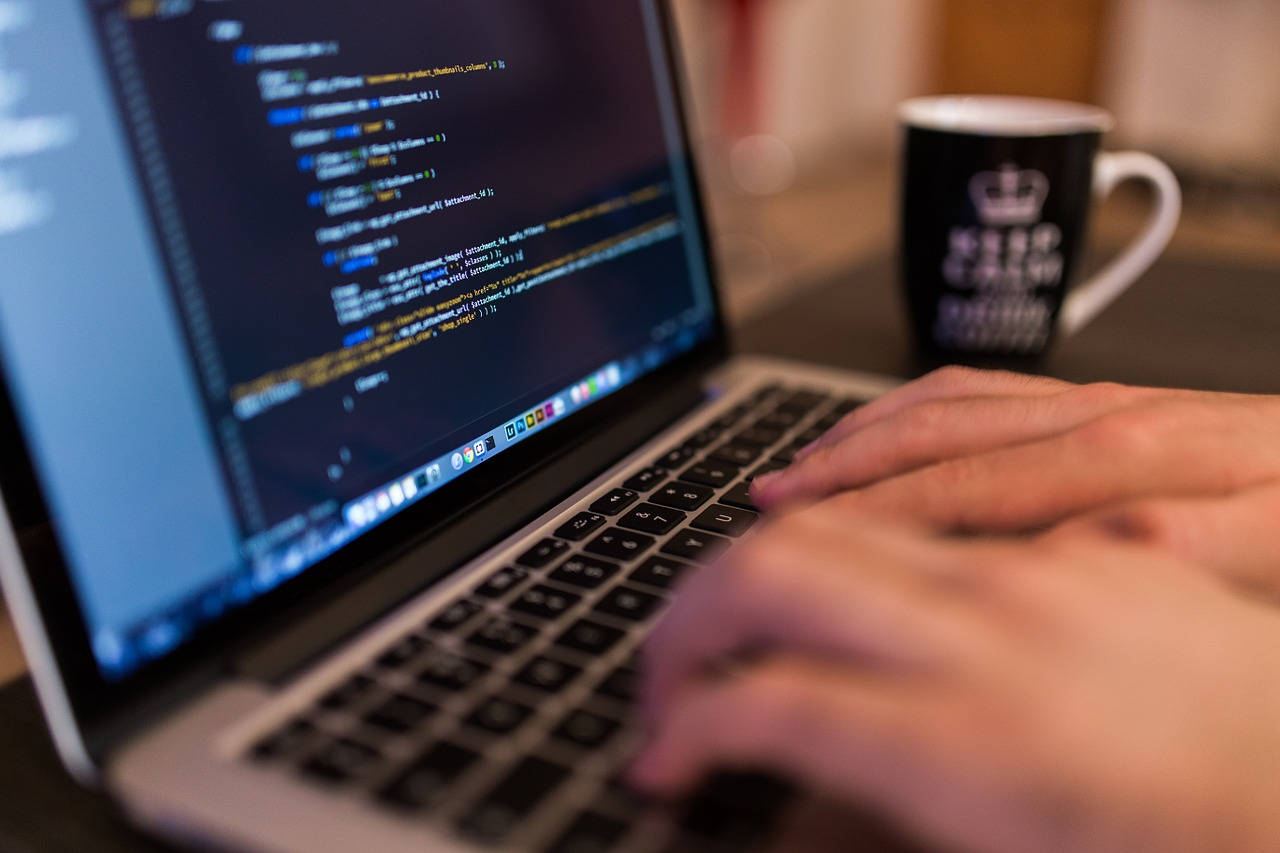
\includegraphics[width=6cm]{../../images/hands_on.jpg}};
  \end{tikzpicture}
\end{pframe}


\subsection{Teachers}
\begin{pframe}
 \begin{minipage}[t]{0.5\textwidth}
  \begin{itemize}
   \item Mark Santcroos \\
     \hrefcc{emailc}{m.a.santcroos@lumc.nl}
   \item Jonathan Vis \\
     \hrefcc{emailc}{j.k.vis@lumc.nl}
   \item Ruben Vorderman \\
     \hrefcc{emailc}{r.h.p.vorderman@lumc.nl}
   \item Redmar van den Berg \\
     \hrefcc{emailc}{r.r.van\_den\_berg@lumc.nl}
   \item Mihai Lefter\\
    \hrefcc{emailc}{m.lefter@lumc.nl}
  \end{itemize}
 \end{minipage}
  \begin{tikzpicture}[remember picture,overlay]
    \node[xshift=-5.0cm,yshift=-6.0cm] at (current page.north east)
    {\includesvg[inkscapelatex=false,width=7cm]{../../images/class.svg}};
  \end{tikzpicture}
\end{pframe}


\subsection{Program}
\begin{pframe}
 \begin{center}
  \includesvg[inkscapelatex=false,width=0.95\textwidth]{../../images/program.svg}
 \end{center}
\end{pframe}


\subsection{Software requirements}
\begin{pframe}
 \begin{itemize}
  \item Anaconda:
  \begin{itemize}
   \item Python $3.7$.
   \item Comes with all that's required:
   \begin{itemize}
    \item Python interpreter.
    \item Jupyter Notebook.
    \item Libraries: NumPy, Panda,\\
    matplotlib, Bokeh, Biopython, ...
   \end{itemize}
   \item \hrefc{emailc}{http://docs.anaconda.com/anaconda/install/}{Installation instructions}.
  \end{itemize}
  \bigskip
  \item Git:
  \begin{itemize}
   \item \hrefc{emailc}{https://git-scm.com/book/en/v2/Getting-Started-Installing-Git}{Installation instructions}.
  \end{itemize}
 \end{itemize}
 \begin{tikzpicture}[remember picture,overlay]
   \node[xshift=-4.5cm,yshift=-5.5cm] at (current page.north east)
   {
\includegraphics[width=3cm]{../../images/requirements_logos.pdf}};
 \end{tikzpicture}
\end{pframe}


\subsection{Assignments}
\begin{pframe}
 \begin{itemize}
  \item We make use of GitHub Classroom.
  \begin{itemize}
   \item GitHub account required.
   \item Receive link with assignment repository.
  \end{itemize}
  \item Own forked repository to work on:
  \begin{itemize}
   \item Clone it.
   \item Code it.
   \item Push it.
  \end{itemize}
  \item Direct file upload to repository\\
  is also possible.
 \end{itemize}
 \begin{tikzpicture}[remember picture,overlay]
    \node[xshift=-4.5cm,yshift=-6.5cm] at (current page.north east)
    {
\includegraphics[width=6cm]{../../images/assignments.jpg}};
  \end{tikzpicture}
\end{pframe}


\subsection{Getting help}
\begin{pframe}
 \begin{itemize}
  \item Ask a teacher (we will be around in the afternoon).
  \item If it's private, mail one of the teachers.
 \end{itemize}
 \begin{center}
  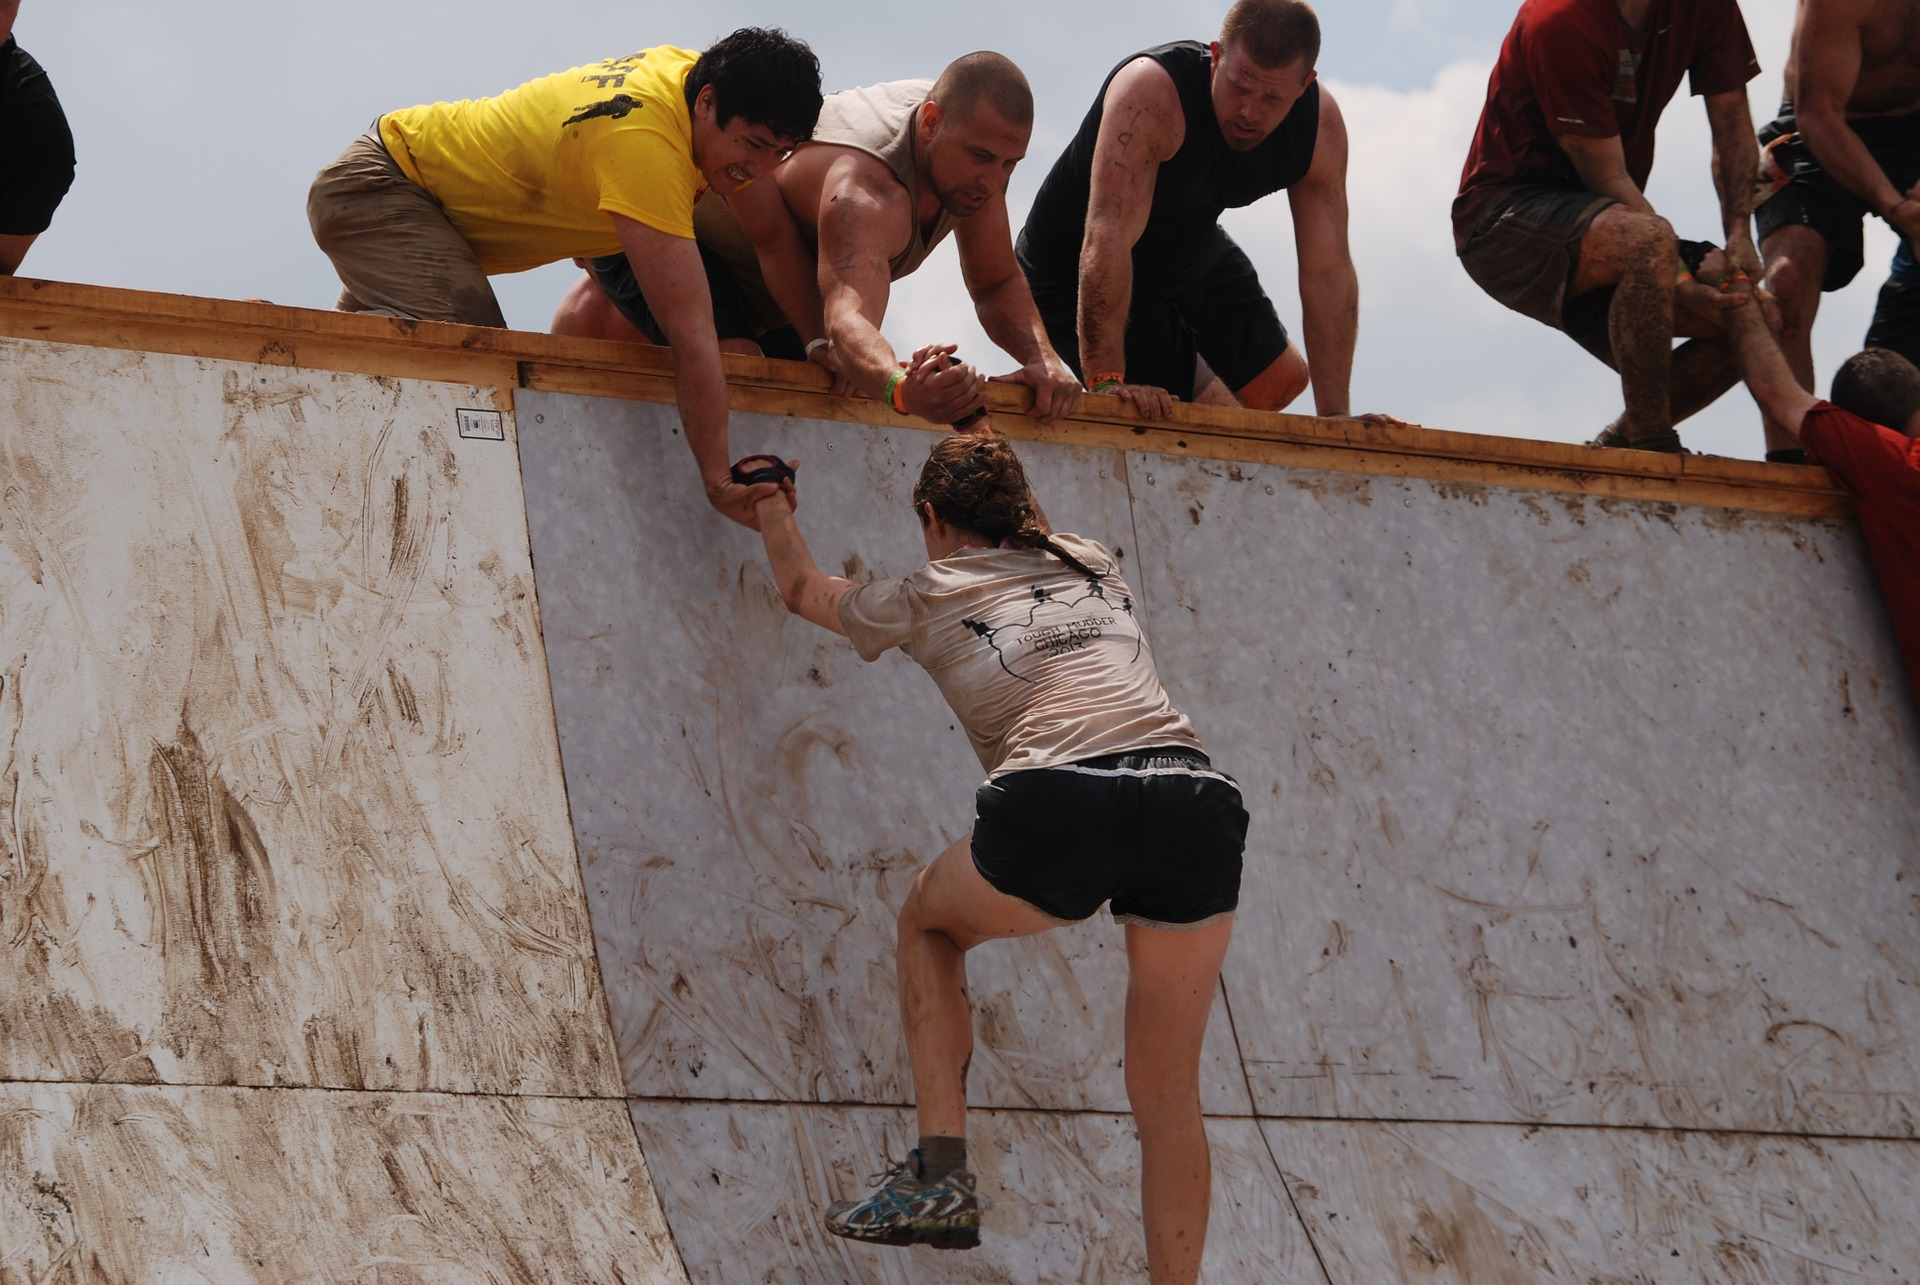
\includegraphics[width=0.54\textwidth]{../../images/help.jpg}
 \end{center}
\end{pframe}


\section{About Python}

\subsection{History}
\begin{pframe}
 \begin{itemize}
  \item Created early 90's by Guido van Rossem at CWI.
  \begin{itemize}
   \item Name: Monty Python.
  \end{itemize}
  \item Design is driven by code readability.
 \end{itemize}
 \begin{tikzpicture}[remember picture,overlay]
   \node[xshift=-4.5cm,yshift=-6.5cm] at (current page.north east)
   {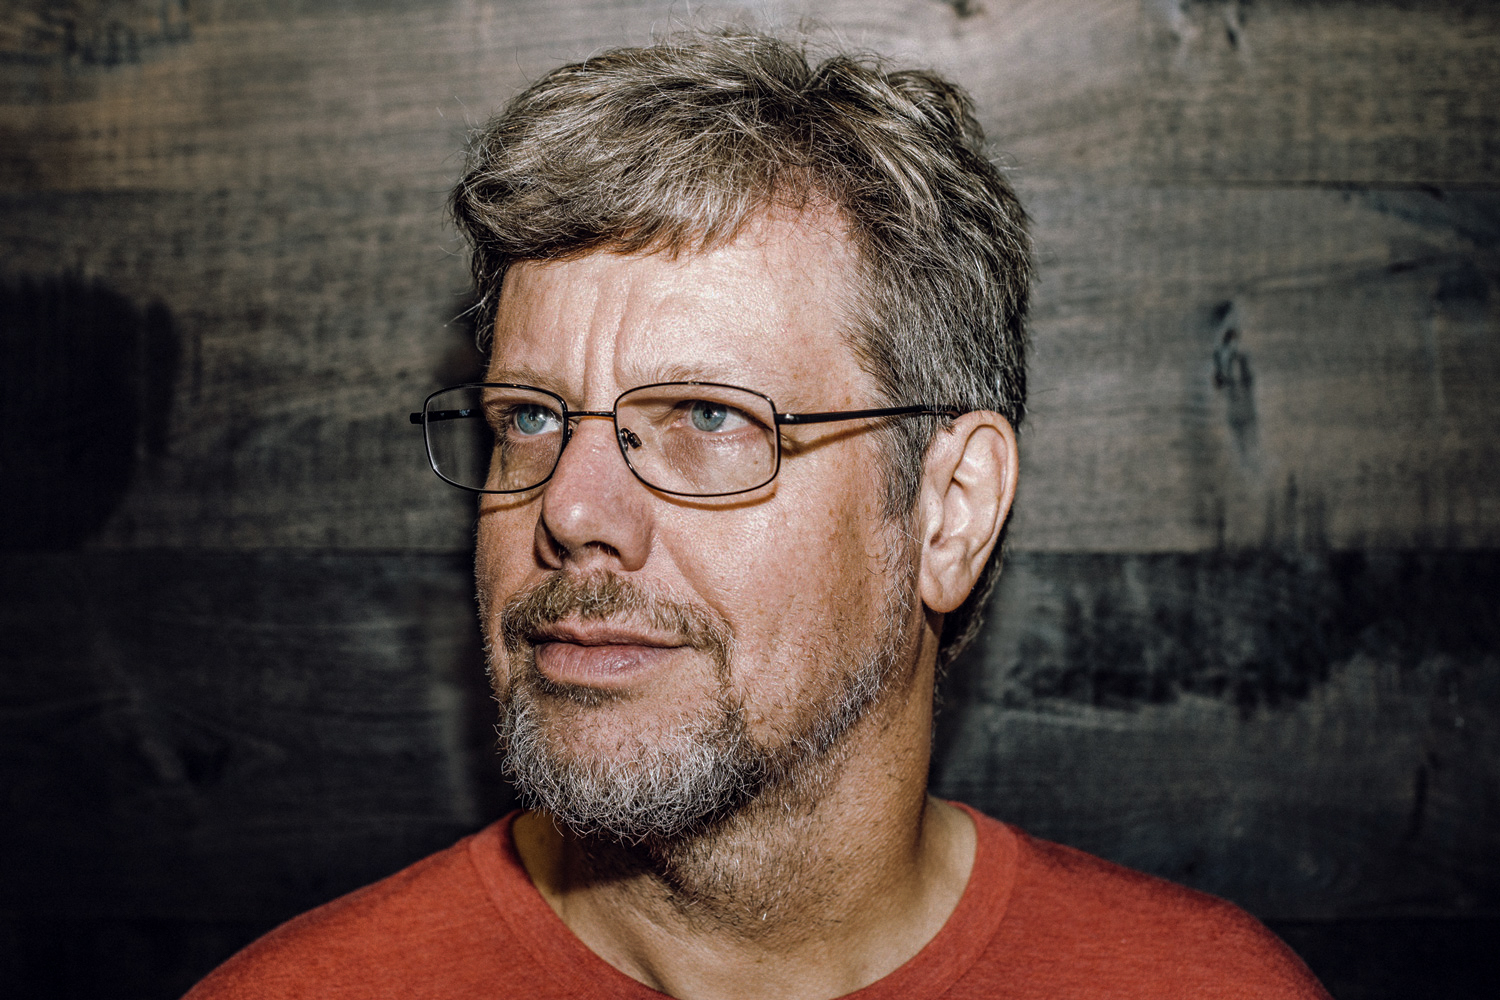
\includegraphics[width=6cm]{../../images/Guido.jpg}};
 \end{tikzpicture}
 \begin{tikzpicture}[remember picture,overlay]
   \node[xshift=-11.5cm,yshift=-6.5cm] at (current page.north east)
   {\includesvg[inkscapelatex=false,width=6cm]{../../images/cwi.svg}};
 \end{tikzpicture}
\end{pframe}


\subsection{Features}
\begin{pframe}
 \begin{itemize}
  \item General purpose, high-level programming language.
  \item Interpreted, no separate compilation step needed.
  \item Imperative and object-oriented programming.
  \begin{itemize}
   \item And some functional programming.
  \end{itemize}
  \item Dynamic type system.
  \item Automatic memory management.
 \end{itemize}
 We'll come back to most of this.
 \begin{tikzpicture}[remember picture,overlay]
    \node[xshift=-4.5cm,yshift=-6.5cm] at (current page.north east)
    {
\includegraphics[width=6cm]{../../images/abstract.jpg}};
  \end{tikzpicture}
\end{pframe}


\subsection{Why Python?}
\begin{pframe}
 \begin{itemize}
  \item Widely used with a large community.
 \end{itemize}
 \vspace{-0.5cm}
 \begin{center}
  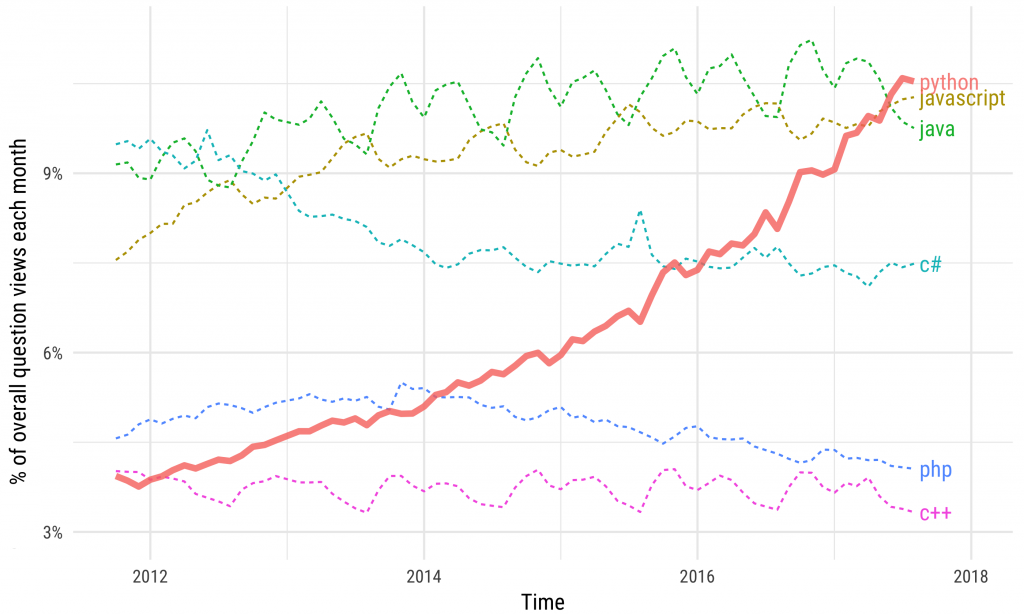
\includegraphics[width=0.70\textwidth]{../../images/growth_major_languages-1-1024x878_stackoverflow_c.png}
  \tiny{https://stackoverflow.blog/2017/09/06/incredible-growth-python/}
 \end{center}
\end{pframe}

\begin{pframe}
 \begin{itemize}
  \item Widely used with a large community.
 \end{itemize}
 \vspace{-0.5cm}
 \begin{center}
  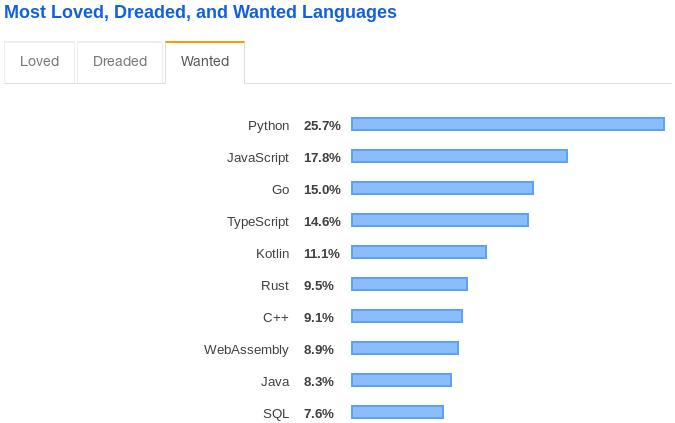
\includegraphics[width=0.70\textwidth]{../../images/stackoverflow_most_wanted_2019.png}\\
  \tiny{https://insights.stackoverflow.com/survey/2019/\#most-loved-dreaded-and-wanted}
 \end{center}
\end{pframe}

\begin{pframe}
 \begin{itemize}
  \item Widely used with a large community.
 \end{itemize}
 \vspace{-0.5cm}
 \begin{center}
  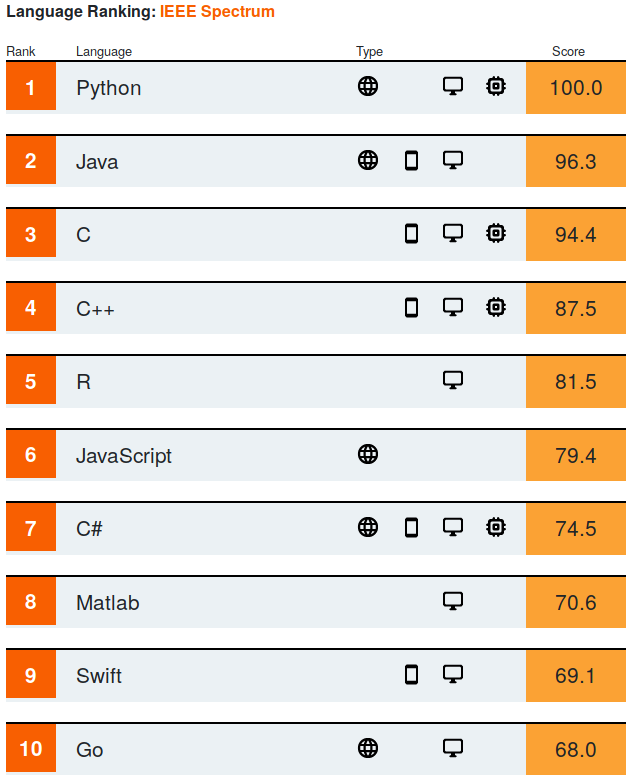
\includegraphics[width=0.35\textwidth]{../../images/ieee_programming_languages_top_2019.png}\\
  \tiny{https://spectrum.ieee.org/computing/software/the-top-programming-languages-2019}
 \end{center}
\end{pframe}

\begin{pframe}
 \begin{itemize}
  \item Widely used with a large community.
  \item Rich scientific libraries.
  \item Many other libraries available.
  \item Readable and low barrier to entry.
 \end{itemize}
 \begin{tikzpicture}[remember picture,overlay]
    \node[xshift=-4.5cm,yshift=-6.5cm] at (current page.north east)
    {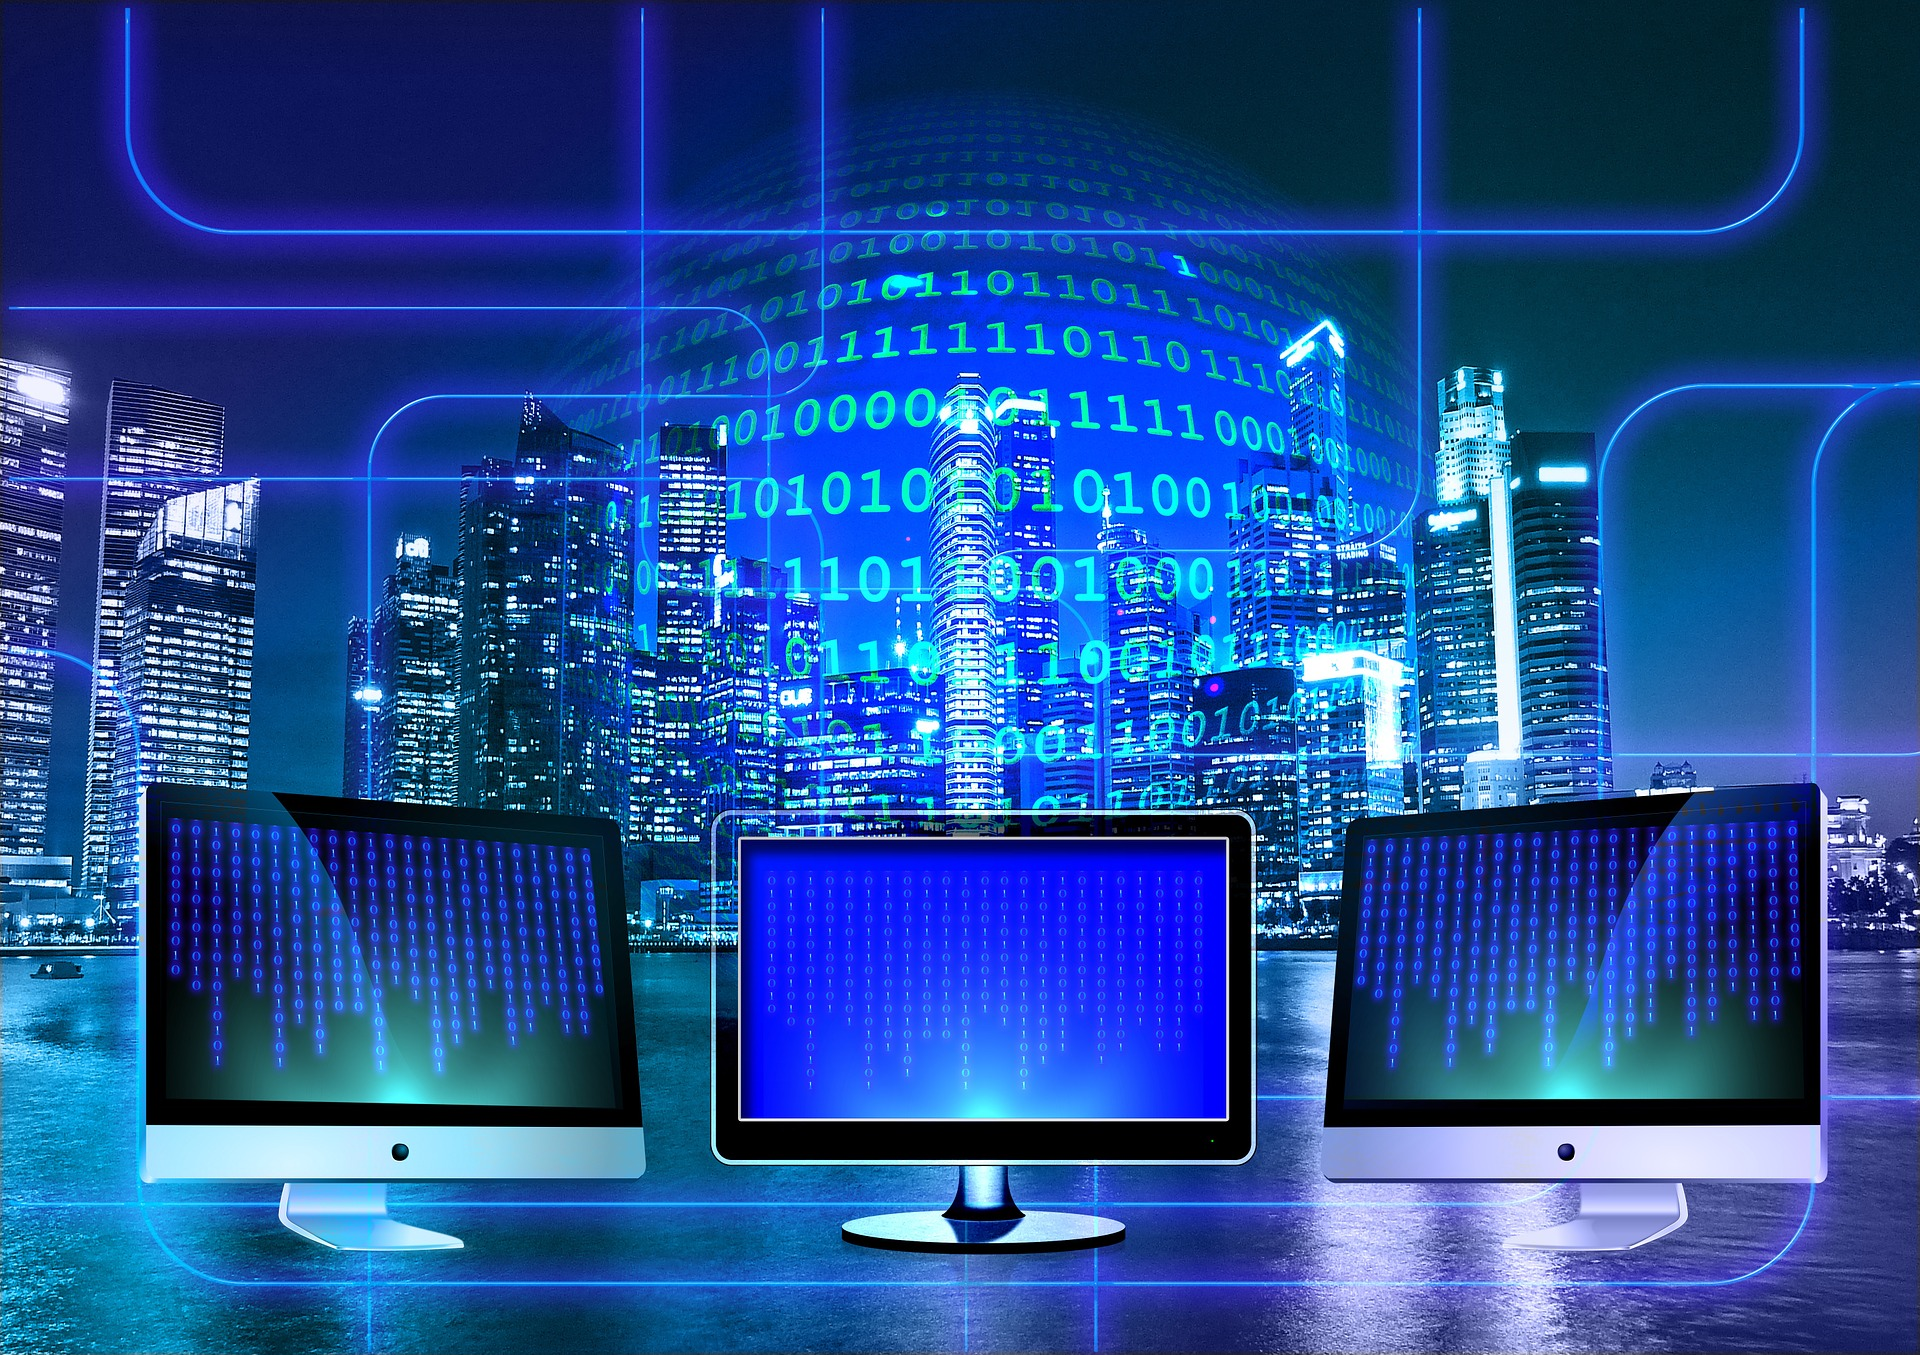
\includegraphics[width=6cm]{../../images/widely.jpg}};
  \end{tikzpicture}
\end{pframe}

\subsection{Python 2 versus Python 3}
\begin{pframe}
 \begin{itemize}
  \item Python 2.7 is the last Python 2.
  \item Python 3 is backwards incompatible.
  \item Some libraries don't support it yet.
  \item Some Python 3 features are backported in Python 2.7.
  \item Python 2.7 will not be maintained past 2020.
 \end{itemize}
  We'll use Python 3.7 for this course.
\end{pframe}


\section{Running Python code}

\begin{pframe}
\vspace{-0.5cm}
\begin{minipage}[t]{0.47\textwidth}
  Interactively:
  {\small
  \begin{itemize}
    \item Statement by statement, directly in the interpreter.
  \end{itemize}}
  \pause
  \begin{terminal}
  {\tiny \color{white}{
   \begin{lstlisting}[frame=,style=,numbers=none,aboveskip=-0.1cm,belowskip=-0.1cm]
$ python
Python 3.7 (default, Nov 26 2019, 10:23:46)
[GCC 5.4.0 20160609] on linux
Type "help", "copyright", "credits" or
"license" for more information.
>>> print('Hello world')
Hello world
>>>
  \end{lstlisting}}}
 \end{terminal}
 \pause
 {\small
 \begin{itemize}
  \item Interpreters are great for prototyping.
  \item But not really suitable if you want to share or release code.
 \end{itemize}}
 \end{minipage}\qquad%
 \begin{minipage}[t]{0.47\textwidth}
  \pause
  \vspace{-0.3cm}
  Non-interactively:
  {\small
  \begin{itemize}
   \item By editing a file and running the code afterwards.
  \end{itemize}}
  \pause
  \begin{pythonfile}{first\_script.py}
   \begin{minted}[linenos]{python}
print("Hello world!")
   \end{minted}
  \end{pythonfile}
  \pause
  \begin{terminal}
   {\tiny \color{white}{
   \begin{lstlisting}[frame=,style=,numbers=none,aboveskip=-0.1cm,belowskip=-0.1cm]
$ python first_script.py
Hello world
$
   \end{lstlisting}}}
  \end{terminal}
 \end{minipage}
\end{pframe}

\subsection{The IPython interpreter}
\begin{pframe}
  Similar to the standard Python interpreter, but with:
  \begin{itemize}
    \item syntax highlighting;
    \item tab completion;
    \item cross-session history;
    \item etc.
  \end{itemize}
  \medskip

  \begin{terminal}
  \color{white}{
   \begin{lstlisting}[frame=,style=,numbers=none,aboveskip=-0.1cm]
$ ipython
Python 3.7 (default, Nov 12 2018, 13:43:14)
Type 'copyright', 'credits' or 'license' for more information
IPython 6.1.0 -- An enhanced Interactive Python. Type '?' for help.
  \end{lstlisting}}
  \begin{pythonin}{python}
  \end{pythonin}
  \addtocounter{cntr}{-1}
 \end{terminal}
\end{pframe}


\section{Python as a calculator}

\subsection{Integers}
\begin{pframe}
 \begin{ipython}
  \begin{pythonin}{python}
17
  \end{pythonin}
  \begin{pythonout}
17
  \end{pythonout}
  \\

  \begin{pythonin}{python}
(17 + 4) * 2 - 10
  \end{pythonin}
  \begin{pythonout}
32
  \end{pythonout}
  \\

  \begin{pythonin}{python}
14 // 4  # floor division - quotient
  \end{pythonin}
  \begin{pythonout}
3
  \end{pythonout}
  \\

  \begin{pythonin}{python}
14 % 4   # modulus - remainder
  \end{pythonin}
  \begin{pythonout}
2
  \end{pythonout}
  \\

  \begin{pythonin}{python}
2 ** 3   # exponentiation
  \end{pythonin}
  \begin{pythonout}
8
  \end{pythonout}
 \end{ipython}
\end{pframe}


\subsection{Floating point numbers}
\begin{pframe}
 \begin{ipython}
  \begin{pythonin}{python}
3.2 * 18 - 2.1
  \end{pythonin}
  \begin{pythonout}
55.5
  \end{pythonout}
  \\

  \begin{pythonin}{python}
36 / 5
  \end{pythonin}
  \begin{pythonout}
7.2
  \end{pythonout}
 \end{ipython}
\end{pframe}


\begin{pframe}
Scientific notation:
\begin{ipython}
  \begin{pythonin}{python}
1.3e20 + 2
  \end{pythonin}
  \begin{pythonout}
1.3e+20
  \end{pythonout}
  \\

  \begin{pythonin}{python}
1.3 * 10**20
  \end{pythonin}
  \begin{pythonout}
1.3e+20
  \end{pythonout}
 \end{ipython}
\end{pframe}


\section{Variables}

\begin{pframe}
 \vspace{-0.75cm}
 \begin{itemize}
  \item Names (identifiers) used to reference values. Can consist of:
  \begin{itemize}
   \item the uppercase and lowercase letters \emp{A} through \emp{Z};
   \item the underscore \emp{\_};
   \item the digits \emp{0} through \emp{9}, except for the first character.
  \end{itemize}
  \item Notes:
  \begin{itemize}
   \item Python is case sensitive.
   \item \hrefc{linkc}{https://docs.python.org/3.7/reference/lexical_analysis.html\#keywords}{Reserved words} (\emp{if}, \emp{then}, \emp{for}, etc.) are not be employed.
  \end{itemize}
 \end{itemize}

 \begin{ipython}
  \begin{pythonin}{python}
a = 17
  \end{pythonin}
  \\
  \begin{pythonin}{python}
leiden_population = 123856
  \end{pythonin}
  \\
  \begin{pythonin}{python}
f18_speed = 1.8
  \end{pythonin}
 \end{ipython}
\end{pframe}


\begin{pframe}
 \vspace{-0.75cm}
 \begin{itemize}
  \item No need to declare them first or define the type.
  \item However, you do need to give variables values before you use them.
 \end{itemize}

 \begin{ipython}
  \begin{pythonin}{python}
a = 17
  \end{pythonin}
  \\
  \begin{pythonin}{python}
c = a + b
  \end{pythonin}
  \begin{pythonerr}{python}
---------------------------------------------------------------------------
NameError                                 Traceback (most recent call last)
<ipython-input-2-1674f6151070> in <module>
----> 1 c = a + b

NameError: name 'b' is not defined
  \end{pythonerr}
 \end{ipython}
\end{pframe}


\section{Python's type system}

\subsection{Every value has a type}
\begin{pframe}
 \begin{itemize}
  \item View it using \mintinline{python}{type}.
 \end{itemize}

 \begin{ipython}
  \begin{pythonin}{python}
type(27)
  \end{pythonin}
  \begin{pythonout}
int
  \end{pythonout}
  \\

  \begin{pythonin}{python}
type(3 * 2)
  \end{pythonin}
  \begin{pythonout}
int
  \end{pythonout}
  \\

  \begin{pythonin}{python}
type(3 / 2)
  \end{pythonin}
  \begin{pythonout}
float
  \end{pythonout}
  \\

  \begin{pythonin}{python}
type(a)
  \end{pythonin}
  \begin{pythonout}
int
  \end{pythonout}
 \end{ipython}
\end{pframe}


\subsection{Some operations are defined on more than one type}
\begin{pframe}
 \begin{itemize}
  \item Possibly with different meanings.
 \end{itemize}

 \begin{ipython}
  \begin{pythonin}{python}
type(3 * 2.0)
  \end{pythonin}
  \begin{pythonout}
float
  \end{pythonout}
  \\

  \begin{pythonin}{python}
drinks = 'beer' * 5 + 'whiskey'
  \end{pythonin}
  \\
  \begin{pythonin}{python}
drinks
  \end{pythonin}
  \begin{pythonout}
'beerbeerbeerbeerbeerwhiskey'
  \end{pythonout}
  \\

  \begin{pythonin}{python}
type(drinks)
  \end{pythonin}
  \begin{pythonout}
str
  \end{pythonout}
 \end{ipython}
\end{pframe}


\subsection{Dynamic typing}
\begin{pframe}
 \begin{itemize}
  \item At runtime variables can be assigned values of different types.
 \end{itemize}

 \begin{ipython}
  \begin{pythonin}{python}
a
  \end{pythonin}
  \begin{pythonout}
17
  \end{pythonout}
  \\

  \begin{pythonin}{python}
type(a)
  \end{pythonin}
  \begin{pythonout}
int
  \end{pythonout}
  \\

  \begin{pythonin}{python}
a = 'spezi'
  \end{pythonin}
  \\
  \begin{pythonin}{python}
type(a)
  \end{pythonin}
  \begin{pythonout}
str
  \end{pythonout}
 \end{ipython}
\end{pframe}


\subsection{Strongly typed}
\begin{pframe}
 \begin{itemize}
  \item Operations on values with incompatible types are forbidden.
 \end{itemize}

 \begin{ipython}
  \begin{pythonin}{python}
'beer' + 34
  \end{pythonin}
  \begin{pythonerr}{python}
---------------------------------------------------------------------------
TypeError                                 Traceback (most recent call last)
<ipython-input-17-ec918fbfdf41> in <module>()
----> 1 'beer' + 34

TypeError: Can't convert 'int' object to str implicitly
  \end{pythonerr}
 \end{ipython}
\end{pframe}


\section{Ipython magics}

\begin{pframe}
 \begin{ipython}
  \begin{pythonin}{python}
%save introduction 1-25
  \end{pythonin}
  \begin{pythonoutnonumber}
The following commands were written to file 'introduction.py':\\
...
  \end{pythonoutnonumber}\\
  \begin{pythonin}{python}
%run introduction.py
  \end{pythonin}
  \\

  \begin{pythonin}{python}
exit
  \end{pythonin}
 \end{ipython}

 Documentation of all the magics is to be found
  \hrefc{linkc}{https://ipython.readthedocs.io/en/stable/interactive/magics.html}{here}.
\end{pframe}


\section{Hands on!}
\begin{pframe}
 \vspace{-0.5cm}
 \begin{enumerate}
  \item We've seen that \mintinline{python}{b = 2} is legal.
  \begin{enumerate}[a.]
   \item What about \mintinline{python}{2 = b}?
   \item How about \mintinline{python}{a = b = 1}?
  \end{enumerate}
  \item In math notation you can multiply $x$ and $y$ like this: $xy$. What
  happens if you try that in Python?
  \item How many seconds are there in $42$ minutes and $42$ seconds?
  \item How many miles are there in $16$ kilometers? ($1$ mile = $1.61$ km)
  \item Let's assume that you run a $42$ km race in $4$ hours $42$ minutes and
  $42$ seconds.
  \begin{enumerate}[a.]
   \item What is your average pace (time per mile in minutes and seconds)?
   \item What is your average speed in miles per hour?
  \end{enumerate}
  \item Use string operations to reference \mintinline{python}{'tra la la la'}
  in a variable named \mintinline{python}{song}.
  \item If an article costs $249$ Euros including the $19\%$ Value Added Tax
  (VAT), what is the actual VAT amount in Euros for the corresponding article?
 \end{enumerate}
\end{pframe}


% Make the acknowledgements slide.
\makeAcknowledgementsSlide{
  \begin{tabular}{ll}
    Martijn Vermaat\\
    Jeroen Laros\\
    Jonathan Vis
  \end{tabular}
}

\end{document}
